%%%%%%%%%%%%%%%%%%%%%%%%%%%%%%%%%%%%%%%%%%%%%%%%%%%%%%%%%%%%%%%%%%%%%%
% Lớp 11 | Hàm số mũ và hàm số lôgarít | Hàm số mũ. Hàm số lôgarít
% Dạng 1D6?3-4: So sánh các luỹ thừa và lôgarít
% Số câu: 15  (sinh tự động bởi tach_cau.py; từ nay thầy sửa trực tiếp file này)
%%%%%%%%%%%%%%%%%%%%%%%%%%%%%%%%%%%%%%%%%%%%%%%%%%%%%%%%%%%%%%%%%%%%%%

%%%%%%%%%%%%%%%% TRẮC NGHIỆM 4 PHƯƠNG ÁN %%%%%%%%%%%%%%%%

% nguồn: Ok_TracNghiemLop11_Lan1
\begin{ex}%[1D6N3-4]%[ma:35cd79a0]
	Mệnh đề nào sau đây là  đúng?
	\choice 
		 {$2024^{-99}>2024^{-98}$}
		 {$(0,2024)^{999}>(0,2024)^{998}$}
		 {\True $2024^{99}>2024^{98}$}
		{$2024^{99}>2024^{100}$} 
	\loigiai{ 
		Mệnh  đề đúng $2024^{99}>2024^{98}$.
	 }
\end{ex}

% nguồn: Ok_Toan11_TracNghiem_Lan2
\begin{ex}%[1D6H3-4]%[ma:89255772]
	Cho $a$ và $b$ là các số thực dương tùy ý. Nếu $a^2>a^3$ và  $\log_b\dfrac{1}{3}<\log_b\dfrac{1}{4}$ thì
	 \choice
		{\True  $a>1$, $0<b<1$}
		{$0<a<1$,  $0<b<1$}
		{$a>1$, $b>1$} 
		 {$0<a<1$, $b>1$}
	\loigiai{ 
		Ta có $\dfrac{1}{2}>\dfrac{1}{3}$  mà $a^2>a^3$ nên $a>1$.\\
		Mặt khác, $\dfrac{1}{3}>\dfrac{1}{4}$ mà  $\log_b\dfrac{1}{3}<\log_b\dfrac{1}{4}$ nên $0<b<1$.
	} 
\end{ex}

% nguồn: Ok_TracNghiemLop11_Lan1
\begin{ex}%[1D6H3-4]%[ma:f1418595]
	Cho  $a>1$. Mệnh đề nào sau đây là đúng?
	 \choice
		{\True $a^{-\sqrt{3}} >  \dfrac{1}{a^{\sqrt{5}}}$}
		{$a^{\tfrac{1}{3}}  > \sqrt{a}$}
		{$\dfrac{\sqrt[3]{a^2}}{a} >  1$}
		{$\dfrac{1}{a^{2016}} <  \dfrac{1}{a^{2017}}$}
	\loigiai{ 
		Vì $a >  1$; $-\sqrt{3} >-\sqrt{5}$ $\Rightarrow a^{-\sqrt{3}} > a^{-\sqrt{5}} \Leftrightarrow a^{-\sqrt{3}} > \dfrac{1}{a^{\sqrt{5}}}$.
	 }
\end{ex}

% nguồn: Ok_TracNghiemLop11_Lan1
\begin{ex}%[1D6H3-4]%[ma:0602d3a7]
	Cho $a, b,  c > 0$ và $a > 1$. Trong các khẳng định sau, khẳng định nào là {\bf sai}?
	\choice 
		{\True $\log_a b > c  \Leftrightarrow b > c$}
		{$\log_a  b > \log_a c \Leftrightarrow b > c$}
		{$a^b > a^c \Leftrightarrow b > c$} 
		 {$\log_a b < \log_a c \Leftrightarrow b < c$}
	 \loigiai{
		Vì cơ số $a > 1$ nên 
		\begin{itemize}
			\item $\log_a b > c \Leftrightarrow b > a^c$. Do đó, $\log_a b > c \Leftrightarrow b > c$ là khẳng  định sai.
			\item Các khẳng định còn lại đều đúng. 
		\end{itemize}
	 }
\end{ex}

% nguồn: Ok_TracNghiemLop11_Lan1
\begin{ex}%[1D6H3-4]%[ma:943f499b]
	Cho số  thực $a$ thỏa $a>1$. Mệnh đề nào sau đây \textbf{đúng}?
	 \choice
		{$\sqrt[3]{a^2}>a$} 
		{\True  $a^{-\sqrt{3}}>\dfrac{1}{a^{\sqrt{5}}}$}
		 {$a^{\frac{1}{3}}>\sqrt{a}$}
		 {$\dfrac{1}{a^{2023}}<\dfrac{1}{a^{2024}}$}
	\loigiai{ 
		Ta  có
		\begin{itemize}
			\item  Xét đáp án $\sqrt[3]{a^2}>a$. Vì $\dfrac{2}{3}<1$ nên $\sqrt[3]{a^2}<a$.
			\item Xét đáp án $a^{-\sqrt{3}}>\dfrac{1}{a^{\sqrt{5}}}$. Vì $-\sqrt{3}>-\sqrt{5}$ nên  $a^{-\sqrt{3}}>\dfrac{1}{a^{\sqrt{5}}}$.
			\item  Xét đáp án $a^{\frac{1}{3}}>\sqrt{a}$. Vì $\dfrac{1}{3}<\dfrac{1}{2}$ nên $a^{\frac{1}{3}}<\sqrt{a}$.
			\item Xét đáp án $\dfrac{1}{a^{2023}}<\dfrac{1}{a^{2024}}$. Vì $\dfrac{1}{2023}>\dfrac{1}{2024}$  nên $\dfrac{1}{a^{2023}}<\dfrac{1}{a^{2024}}$.
		\end{itemize}
	 }
\end{ex}

% nguồn: Ok_TracNghiemLop11_Lan1
\begin{ex}%[1D6H3-4]%[ma:1fed369e]
	Cho $a=3^{\sqrt{5}},b=3^2$ và  $c=3^{\sqrt{6}}$ mệnh đề nào dưới đây đúng
	\choice 
		{$a<c<b$} 
		 {$a<b<c$}
		{\True  $b<a<c$}
		{$c<a<b$} 
	\loigiai{ 
	 Ta có $a=3^{\sqrt{5}},b=3^2=3^{\sqrt{4}},c=3^{\sqrt{6}}$ và $\heva{&\sqrt{4}<\sqrt{5}<\sqrt{6} \\&3>1}\Rightarrow b<a<c$.}
\end{ex}

% nguồn: Ok_Toan11_TracNghiem_Lan2
\begin{ex}%[1D6V3-4]%[ma:539c69f6]
	Cho các hàm số $ y=a^x$ và $ y=b^x$ với $ a$, $b$ là những số thực dương khác $ 1 $, có đồ thị như hình vẽ. Đường thẳng $  y=3$ cắt trục tung, đồ thị hàm số $ y=a^x$ và $ y=b^x$ lần lượt tại $ H$, $M$, $N$. Biết rằng $ 2HM=3MN$, khẳng định nào sau đây đúng?
	\begin{center}
		\begin{tikzpicture}[line join = round,line cap = round,>=stealth,font=\footnotesize,scale =1]
				\draw[->] (-2,0)--(0,0)  node[below right]{$O$}--(4.5,0) node[below]{$x$};
				\draw[->] (0,-1)--(0,4.5) node[right]{$y$}; 
				\draw (-2,2)--(4.5,2)  node [right]{$ d $};
				\clip (-2,-1)  rectangle (3,4.5);
				\draw[samples=300,domain=-2.5:4.5,smooth]  plot (\x,{(2)^(\x)});
				 \draw[samples=300,domain=-2.5:4.5,smooth] plot (\x,{(1.5157)^(\x)});
				\path[name path=ab]  (-2,2)--(4.5,2);
				\path[name path=f] plot (\x,{(2)^(\x)}); 
				\path[name path=g] plot (\x,{(1.5157)^(\x)}); 
				\coordinate (H) at  (0,2);
				\path[name intersections={of= ab and  f,by=M}];
				\path[name  intersections={of= ab and g,by=N}];
				\foreach \x/\y in {M/above left,N/below right,H/below left} \fill (\x) node [\y] {$\x$}  circle (1pt);
			\end{tikzpicture}
	\end{center}
	\choice 
		 {$a^5=b^3$}
		{$ 3a=5b$} 
		 {$a^2=b^3$}
		{\True  $a^3=b^5$}
	 \loigiai{
		$ 2HM=3MN\Rightarrow  HM=\dfrac{3}{5}HN$.\\
		 Gọi $ M\left(x_1;3\right)\in y=a^x\Rightarrow{x_1}=\log_a3$.\\
		$  N\left(x_1;3\right)\in y=b^x\Rightarrow{x_2}=\log_b3$.\\
		Khi đó 
	 $$ HM=\dfrac{3}{5}HN\Leftrightarrow{\log_a}3=\dfrac{3}{5}{\log_b}3\Leftrightarrow\dfrac{1}{\log_3a}=\dfrac{3}{5\log_3b}\Leftrightarrow{\log_3}a=\dfrac{5}{3}{\log_3}b\Leftrightarrow a=b^{\tfrac{5}{3}}\Leftrightarrow{a^3}=b^5.$$ }
\end{ex}

% nguồn: Ok_Toan11_TracNghiem_Lan2
\begin{ex}%[1D6V3-4]%[ma:6de4d025]
	Cho số thực dương $a$ khác $1$. Biết rằng bất kì đường thẳng nào song song với trục $Ox$ mà cắt các đồ thị $y=4^x$, $y=a^x$, trục tung lần lượt tại $M$, $N$  và $A$ thì $AN=2AM$. Giá trị của $a$ bằng
	\begin{center}
		\begin{tikzpicture}[line join = round,line cap = round,>=stealth,font=\footnotesize,scale =1]
				\draw[->] (-3,0)--(0,0) node[below right]{$O$}--(3.5,0) node[below]{$x$}; 
				\draw[->] (0,-1)--(0,4.5) node[right]{$y$}; 
				\draw (-3,3)--(3.5,3) node  [right]{$ d $};
				\clip (-3,-1) rectangle  (3,4.5);
				\draw[samples=300,domain=-2.5:4.5,smooth]  plot (\x,{(4)^(\x)});
				\draw[samples=300,domain=-2.5:4.5,smooth] plot  (\x,{(0.5)^(\x)});
				\path[name path=ab]  (-2,3)--(4.5,3);
				 \path[name path=f] plot (\x,{(4)^(\x)});
				\path[name path=g]  plot (\x,{(0.5)^(\x)});
				\coordinate  (A) at (0,3);
				\path[name intersections={of= ab and f,by=M}]; 
				\path[name intersections={of= ab  and g,by=N}];
				\foreach \x/\y in {M/below right,N/below left,A/above left} \fill (\x) node [\y] {$\x$}  circle (1pt);
			\end{tikzpicture}
	\end{center}
	\choice 
		{$\dfrac{1}{3}$} 
		{$\dfrac{\sqrt 2}{2}$} 
		{$\dfrac{1}{4}$} 
		{\True $\dfrac{1}{2}$} 
	 \loigiai{
		Giả sử $A\left(0;t\right)$,  $N\left(\log_at;t\right)$, $M\left(\log_4t;t\right)$. Thì $AN=-\log_a t$, $AM=\log_4t$.\\
	Theo giả thiết $AN=2AM\Rightarrow-\log_a  t=2\log_4 t\Leftrightarrow\log_{a^{-1}}t=\log_2 t\Leftrightarrow a=\dfrac{1}{2}$.}
\end{ex}

% nguồn: Ok_Toan11_TracNghiem_Lan2
\begin{ex}%[1D6V3-4]%[ma:6b5f59ff]
	Cho $a$, $b$ là các số thực dương khác $1$, đường thẳng $d$ song song trục hoành cắt trục tung, đồ thị hàm số $y=a^x$, đồ thị hàm số $y=b^x$ lần lượt tại $H$, $M$, $N$. Biết $HM=3MN$. Mệnh đề nào sau đây đúng? 
	\begin{center}
		\begin{tikzpicture}[line join = round,line cap = round,>=stealth,font=\footnotesize,scale =1]
				\draw[->] (-2,0)--(0,0) node[below right]{$O$}--(4.5,0) node[below]{$x$}; 
				\draw[->] (0,-1)--(0,4.5)  node[right]{$y$};
				\draw (-2,2)--(4.5,2)  node [right]{$d$};
				\clip  (-2,-1) rectangle (3,4.5);
				\draw[samples=300,domain=-2.5:4.5,smooth] plot (\x,{(2)^(\x)}); 
				\draw[samples=300,domain=-2.5:4.5,smooth]  plot (\x,{(1.68)^(\x)});
				 \path[name path=ab] (-2,2)--(4.5,2);
				\path[name path=f] plot (\x,{(2)^(\x)}); 
				\path[name path=g] plot (\x,{(1.68)^(\x)}); 
				\coordinate (H)  at (0,2);
				\path[name intersections={of= ab  and f,by=M}];
				 \path[name intersections={of= ab and g,by=N}];
				 \coordinate (E) at ($(0,0)!(M)!(4,0)$);
				\coordinate (F) at ($(0,0)!(N)!(4,0)$); 
				\foreach \x/\y in {M/above left,N/below right,H/below left} \fill (\x) node [\y] {$\x$}  circle (1pt);
				 \fill (E) node [below] {$x_M$} circle (1pt);
				\fill (F) node [below right]  {$x_N$} circle (1pt);
				\draw[dashed] (M)--(E) 
					(N)--(F); 
			\end{tikzpicture}
	\end{center}
	 \choice
		{$4a=3b$} 
		 {\True $b^4=a^3$}
		{$b^3=a^4$} 
		 {$3a=4b$}
	 \loigiai{
		Đường thẳng $d$ cắt đồ thị hàm số $ y=a^x$ tại điểm  $ M(x_M;y_M)$ $\Rightarrow{y_M}=a^{x_M}$.\\
		Đường thẳng $ d$ cắt  đồ thị hàm số $ y=b^x$ tại điểm $ N(x_N;y_N)$ $\Rightarrow{y_N}=b^{x_N}$.\\
		 Mà $y_M=y_N$ $\Rightarrow{a^{x_M}}=b^{x_N}$.\\
	Ta có $  HM=3MN$ $\Rightarrow HM=\dfrac{3}{4}HN$ $\Rightarrow{x_M}=\dfrac{3}{4}{x_N}$ $\Rightarrow{a^{\tfrac{3}{4}{x_N}}}=b^{x_N}$ $\Leftrightarrow{a^{\tfrac{3}{4}}}=b$ $\Leftrightarrow{a^3}=b^4$.}
\end{ex}

% nguồn: Ok_Toan11_TracNghiem_Lan2
\begin{ex}%[1D6V3-4]%[ma:8301e3c8]
	Biết đồ thị hàm số $ y=f(x)$  đối xứng với đồ thị hàm số $ y=a^x$ $(a > 0$, $a\ne 1)$ qua điểm $ I\left(1;1\right)$. Giá trị của biểu thức $ f\left(2+\log_a\dfrac{1}{2\,022}\right)$ bằng
	 \choice
		{$-2\,022$} 
		 {$ 2\,021$}
		 {$ 2\,022$}
		{\True $-2\,020$} 
	\loigiai{ 
		\begin{center}
			\begin{tikzpicture}[line join = round,line cap = round,>=stealth,font=\footnotesize,scale =1]
					 \draw[->] (-2,0)--(0,0) node[below right]{$O$}--(3.5,0) node[below]{$x$};
					 \draw[->] (0,-2)--(0,3.5) node[right]{$y$};
					\draw[dashed](-2,-2)--(3.5,3.5); 
					\clip (-2,-2) rectangle (3.5,3.5); 
					 \draw[samples=300,domain=-2.5:4.5,smooth] plot (\x,{(2)^(\x)});
					\draw[samples=300,domain=0.05:4.5,smooth]  plot (\x,{(ln (\x))/(ln (2))});
				\end{tikzpicture}
		\end{center}
		Đồ  thị đối xứng với đồ thị hàm số $ y=a^x$ $\left(C_1\right)$ là đồ thị hàm số $ y=\log_ax$ $\left(C_2\right)$.\\
		 Gọi $ A\left(x_A;\,y_A\right)\in\left(C_1\right)\Rightarrow B\left(x_B;\,y_B\right)\in\left(C_2\right)$ là điểm đối xứng với điểm $ A$ qua điểm $ I\left(1;\,1\right)$.\\
		 Ta có $\heva{&\dfrac{x_A+x_B}{2}=1\\&\dfrac{y_A+y_B}{2}=1}\Leftrightarrow\heva{&{x_A}+x_B=2&(1)\\
		&{y_A}+y_B=2.&(2)}$\\ 
		Với  $x_B=2+\log_a\dfrac{1}{2\,022}=2+\log_a1-\log_a2\,022=2-\log_a2\,022$.\\
		Từ ta có $x_A+x_B=2\Leftrightarrow{x_A}=\log_a2\,022$. Suy  ra $y_A=a^{\log_a2\,022}=2\,022$.\\
		Từ ta có $y_A+y_B=2\Leftrightarrow{y_B}=2-2\,022=-2\,020$.\\ 
	 Vậy $y_B=f\left(2+\log_a\dfrac{1}{2\,022}\right)=f\left(x_B\right)=-2\,020$.}
\end{ex}


%%%%%%%%%%%%%%%% ĐÚNG/SAI %%%%%%%%%%%%%%%%

% nguồn: Ok_dungsai_lop11_Lan1
\begin{ex}%[1D6N3-4]%[ma:81e78a6c]
 Với $a$, $b$ là các số thực dương bất kì. Xét  tính đúng sai của các mệnh đề sau
 \choiceTF 
  {$\log_{\tfrac{1}{5}}a>\log_{\tfrac{1}{5}}b\Leftrightarrow  a>b$}
  {$\log (3a)<0$} 
  {\True $\log_{5}a>1\Leftrightarrow  a>5$}
  {\True  $\log_{2024}a^3=3\log_{2024}a$}
 \loigiai{ 
 \begin{itemchoice}
  \itemch Vì $\dfrac{1}{5}\in (0;1)$ nên $\log_{\tfrac{1}{5}}a>\log_{\tfrac{1}{5}}b\Leftrightarrow a<b\,\,\,\forall  a,b\in\mathbb{R}^+$.
  \itemch $a>0\Rightarrow 3a>0\Rightarrow \log (3a) >\log 0\Rightarrow\log (3a)>1$. 
  \itemch Vì $5>1$ nên  $\log_{5}a>1\Leftrightarrow a>5$.
  \itemch Áp dụng  công thức $\log_{a}b^M=M\log_{a}b$, ta có $\log_{2024}a^3=3\log_{2024}a$.
 \end{itemchoice}
  }
\end{ex}

% nguồn: Ok_dungsai_lop11_Lan1
\begin{ex}%[1D6N3-4]%[ma:08adbbe6]
 Cho $a^{\frac{3}{4}}>a^{\frac{4}{5}},\log_b\dfrac{1}{2}<\log_b\dfrac{2}{3}$. Khi đó 
  \choiceTF
  {$a>1, 0<b<1$} 
  {$a>1, b>1$} 
   {$0<a<1, 0<b<1$}
  {\True $0<a<1, b>1$} 
 \loigiai{Ta có $\dfrac{3}{4}<\dfrac{4}{5}$, kết hợp  với $a^{\frac{3}{4}}>a^{\frac{4}{5}}$, suy ra $0<a<1$.\\
  Ta có $\dfrac{1}{2}<\dfrac{2}{3}$, kết hợp $\log_b\dfrac{1}{2}<\log_b\dfrac{2}{3}$  suy ra $b>1$.\\
 Vậy  $0<a<1, b>1$.}
\end{ex}

% nguồn: Ok_dungsai_lop11_Lan1
\begin{ex}%[1D6N3-4]%[ma:550dccaf]
 \immini{Cho  ba số thực dương $a$, $b$, $c$ khác $1$. Đồ thị các hàm số $y=a^x$, $y=b^x$, $y=c^x$ được cho trong hình vẽ dưới đây. Mệnh đề nào dưới đây đúng?
  \choiceTF
  {Hai hàm số $y=a^x$ và $y=c^x$ nghịch  biến trên $\mathbb{R}$ }
  {\True Hai hàm  số $y=b^x$ và $y=c^x$ đồng biến trên $\mathbb{R}$ }
  {Từ đồ thị hàm số ta xác định được $c$  là một số dương nhỏ hơn $1$}
  {\True Từ đồ thị hàm số ta xác định được $a<c<b$} }{ 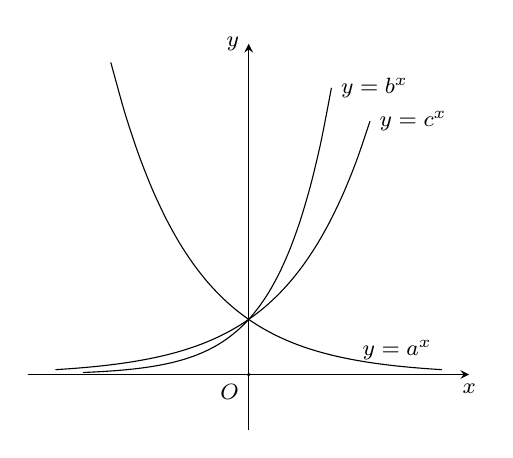
\begin{tikzpicture}[scale=0.7,font=\footnotesize,line join=round,line cap=round,>=stealth,
   declare function={ 
   f (\x)=2^(\x); 
   g (\x)=3^(\x); 
    h (\x)=(1/2)^(\x);
   }] 
   \draw[->] (-4,0)--(4,0) node[below]{$x$};
  \draw[->]  (0,-1)--(0,6) node[left]{$y$};
  \draw[smooth] plot[domain=-3.5:2.2] ({\x},{f (\x)}) node[right]{$y=c^x$}; 
  \draw[smooth] plot[domain=-3:1.5]  ({\x},{g (\x)}) node[right]{$y=b^x$};
  \draw[smooth]  plot[domain=-2.5:3.5] ({\x},{h (\x)}) node[above left]{$y=a^x$};
   \fill (0,0) node[below left]{$O$} circle (1pt);
 \end{tikzpicture}
  } 
 \loigiai{ 
  Ta có  hàm số $y=a^x$ nghịch biến trên $\mathbb{R} \Rightarrow 0<a<1$.\\
  Các hàm  số $y=b^x$ và $y=c^x$ đồng biến trên $\mathbb{R}$ nên $b$, $c >1$.\\
  Ta lại có $\forall x>0$ thì $b^x >c^x \Rightarrow b>c$.\\ 
  Vậy $a<b<c$. 
  \begin{itemchoice}
   \itemch Sai: Hàm số $y=a^x$ nghịch biến  trên $\mathbb{R}$ còn hàm số $y=c^x$ đồng biến trên $\mathbb{R}$.
   \itemch Đúng:  Hai hàm số $y=b^x$ và $y=c^x$ đồng biến trên $\mathbb{R}$.
   \itemch Sai: Từ  đồ thị hàm số ta xác định được $c$ là một số dương lớn hơn $1$.
    \itemch Đúng: Từ đồ thị hàm số ta xác định được $a<b<c$.
  \end{itemchoice}
 } 
\end{ex}

% nguồn: Ok_dungsai_lop11_Lan1
\begin{ex}%[1D6H3-4]%[ma:03b3a4fd]
 Cho $a$, $b$ là các  số thực.
  \choiceTF
  {\True $a >1$  nên $a^{\sqrt{2}} < a^{\sqrt{3}}$}
  {$0<a<1$ nên $\log_a 30 >  \log_a 29{,}7$}
  {$0 <  b < 1$ nên $b^{\tfrac{\sqrt{3}}{4}} < b^{\tfrac{\sqrt{2}}{3}}$}
  {\True $b>1$ nên $\log_b  7 > \log_b 2$}
 \loigiai{ 
  \begin{itemchoice}
   \itemch \textbf{Đúng}. Vì $a>1$ nên hàm số $y=a^x$ đồng biến trên $\mathbb{R}$  và $\sqrt{2} < \sqrt{3}$ nên $a^{\sqrt{2}} < a^{\sqrt{3}}$.
   \itemch \textbf{Sai}.  Vì $0<a<1$ nên hàm số $y = \log_a x$ nghịch biến trên $(0;+\infty)$ và $30 > 29{,}7$ nên $\log_a 30 < \log_a 29{,}7$.
   \itemch \textbf{Sai}. Vì $0<b<1$ nên hàm số $y=b^x$ nghịch biến trên $\mathbb{R}$ và $\dfrac{\sqrt{3}}{4} < \dfrac{\sqrt{2}}{3}$ nên $b^{\tfrac{\sqrt{3}}{4}} >  b^{\tfrac{\sqrt{2}}{3}}$.
   \itemch \textbf{Đúng}. Vì $b>1$ nên hàm số $y = \log_b x$ đồng biến trên $(0;+\infty)$ và $7 > 2$ nên  $\log_b 7 > \log_b 2$.
  \end{itemchoice}
  }
\end{ex}

% nguồn: Ok_dungsai_lop11_Lan1
\begin{ex}%[1D6H3-4]%[ma:baf5fb24]
 Cho  $a>1$.
  \choiceTF
  {\True $a^{6{,}3} >  a^{6{,}2}$}
  {\True  $\log_a (\sqrt{3} - 1) < \log_a (\sqrt{2} + 1)$}
  {$\log_a (\sqrt{3} - 2) < \log_a \sqrt{3}$} 
  {$a^{3} < a^{2\sqrt{2}}$} 
 \loigiai{ 
  Do $a > 1$ nên hàm số $y=a^x$ đồng biến  trên $\mathbb{R}$ và hàm số $y=\log_a x$ đồng biến trên $(0;+\infty)$.
  \begin{itemchoice}
   \itemch \textbf{Đúng}.  Vì $6{,}3 > 6{,}2$.
   \itemch \textbf{Đúng}. Vì $0 < \sqrt{3} -  1 <\sqrt{2} + 1$.
   \itemch \textbf{Sai}. Vì $\sqrt{3} - 2  < 0$.
   \itemch \textbf{Sai}. Vì  $3 > 2\sqrt{2}$.
  \end{itemchoice}
  }
\end{ex}
